Este capítulo apresenta a arquitetura, os componentes e as tecnologias empregadas no
desenvolvimento do \sintonia. São descritos os mecanismos de aquisição dos dados da
balança, o armazenamento e o tratamento das informações, a interface desenvolvida para os
usuários e a integração do assistente virtual baseado em \emph{Small Language Models}
(SLMs). O capítulo descreve também a infraestrutura computacional e os módulos responsáveis
pelo processamento dos dados biométricos, pela geração das interpretações em linguagem
natural e pelas estratégias de privacidade, transparência e aderência às referências
científicas do projeto.

\section{Arquitetura Geral do Sistema}

O \sintonia\ foi concebido como uma plataforma integrada para aquisição, processamento e
interpretação de dados de composição corporal obtidos por bioimpedância segmentada. A
arquitetura combina a leitura direta da balança por Bluetooth, o processamento em servidor
próprio e uma inteligência artificial especializada executada localmente, gerando análises
personalizadas sem depender de serviços em nuvem de terceiros.

A solução tem quatro módulos principais: o dispositivo de aquisição (balança CF577BLE),
lido diretamente pelo navegador pela API Web Bluetooth; o \emph{backend}, responsável por
calcular a composição corporal a partir da impedância bruta; o módulo de IA, baseado em um
SLM local; e a interface de interação com o usuário. O fluxo começa com a medição pelo
usuário: os valores brutos de peso e impedância são lidos pelo navegador e enviados ao
\emph{backend}, que calcula e armazena as métricas. Depois do processamento, os dados vão
para o módulo de IA especializado em bioimpedância, que gera interpretações e recomendações
personalizadas, apresentadas ao usuário em uma interface web responsiva onde ele acompanha
a evolução corporal ao longo do tempo.

Em termos de implementação, o \emph{frontend} é uma aplicação React~18 com Vite~5, React
Router e gráficos em Recharts, distribuída como \emph{Progressive Web App} (PWA)
instalável, com TypeScript adotado de forma gradual e TanStack Query para \emph{cache} e
sincronização dos dados. A interface usa um sistema de \emph{design tokens} (cores,
tipografia e espaçamento), com temas claro e escuro e contraste auditado segundo o WCAG~AA.
A comunicação com a balança é feita pela API Web Bluetooth, diretamente do navegador.

O \emph{backend} é construído em Python com FastAPI, SQLAlchemy~2.0 e Pydantic~2, usando
SQLite em desenvolvimento e PostgreSQL em produção, com migrações de banco versionadas pelo
Alembic. A autenticação usa \emph{JSON Web Token} (JWT), com \emph{access token} curto e
\emph{refresh token} de renovação automática, e os erros seguem um envelope padronizado com
identificador de requisição. O sistema registra \emph{logs} estruturados em JSON para
observabilidade, com remoção de dados pessoais. A implantação usa contêineres Docker
(\emph{backend}, \emph{frontend}, banco, \emph{proxy} Caddy e o modelo de IA via Ollama) e
foi executada em servidor da Universidade de Brasília com aceleração por GPU. As
Figuras~\ref{fig:arquitetura} e~\ref{fig:fluxo} apresentam a arquitetura geral e o fluxo de
processamento do \sintonia.

\figuraplaceholder{Arquitetura completa do sistema \sintonia}{fig:arquitetura}

\figuraplaceholder{Fluxo geral de processamento e interpretação do \sintonia}{fig:fluxo}

\section{Integração com a Balança via Web Bluetooth}

A aquisição é feita diretamente da balança CF577BLE pelo navegador do usuário, pela API Web
Bluetooth, sem depender de servidores em nuvem do fabricante. Quando a balança é ligada (ao
subir nela) e selecionada, o aplicativo estabelece uma conexão BLE e passa a receber os
dados em tempo real. A comunicação segue o protocolo BLE do fabricante (serviço FFF0): o
aplicativo envia o comando de início de medição e o perfil do usuário (sexo, idade e
altura) pela característica de controle e recebe o peso, a frequência cardíaca e as
impedâncias segmentares pela característica de notificação. Toda a troca ocorre localmente,
entre o navegador e a balança.

São lidos os valores brutos de impedância em diferentes segmentos e frequências (20~kHz e
100~kHz), além do peso e da frequência cardíaca. Esses dados crus são enviados ao
\emph{backend}, que calcula a composição corporal. Diferentemente dos aplicativos que
apenas exibem os índices já calculados pelos algoritmos proprietários do aparelho, o
\sintonia\ usa somente a impedância bruta e calcula a composição no próprio servidor, com
equações científicas abertas e validadas contra DXA (Seção~\ref{sec:equacoes}), o que
garante transparência e independência das fórmulas fechadas do fabricante.

Há dois caminhos de aquisição. O preferencial é a leitura direta pela API Web Bluetooth, em
que o próprio navegador pareia com a balança; por exigir contexto seguro (HTTPS), é usado
em ambiente publicado com HTTPS. O caminho alternativo é um agente BLE remoto: um pequeno
processo em Python, executado no computador ligado à balança, que mantém um WebSocket com o
servidor e repassa as leituras, útil quando o navegador do usuário não dispõe de Bluetooth.

\section{Processamento dos Dados de Bioimpedância}

Após a leitura dos dados brutos, inicia-se o processamento das informações corporais, que
garante a consistência dos dados, padroniza as variáveis e prepara as informações para o
módulo de IA. Primeiro, os dados passam por validação: o sistema verifica a integridade dos
registros, a presença dos campos obrigatórios e a coerência dos valores. Depois, os
parâmetros são convertidos para formatos padronizados.

Além dos indicadores que a balança já entrega, o sistema roda rotinas próprias de correção
baseadas na literatura, sobretudo em modelos desenvolvidos para populações brasileiras,
para reduzir vieses dos algoritmos proprietários. Depois desse processamento, os dados são
gravados em banco estruturado, formando o histórico individual de cada usuário, que alimenta
as análises temporais, a identificação de tendências e as recomendações personalizadas. O
sistema também pode incorporar informações de contexto fornecidas pelo usuário, como
alimentação, hidratação e atividade física recentes, que qualificam a interpretação das
medições e alimentam as estratégias de correção.

\section{Desenvolvimento da Interface do Usuário}

A interface do \sintonia\ foi desenvolvida como aplicação web responsiva, utilizável em
computadores, \emph{tablets} e \emph{smartphones} sem instalação por lojas de aplicativos.
A aplicação segue os princípios das \emph{Progressive Web Applications} (PWAs): funciona em
diferentes plataformas, é fácil de atualizar e tem menor custo de distribuição e
manutenção. Novas funcionalidades chegam ao usuário de forma centralizada, sem atualização
manual. A interface foi projetada para ser simples e clara, com os indicadores corporais em
gráficos, tabelas e elementos visuais de leitura fácil. O usuário consulta medições
anteriores, acompanha sua evolução e vê as recomendações do sistema. Além da visualização,
a interface coleta informações complementares (anamnese, hábitos de vida e objetivos de
saúde) que enriquecem as análises. A Figura~\ref{fig:tela}, apresentada na
Seção~\ref{sec:interfaces}, ilustra a tela principal do aplicativo.

\section{Assistente Inteligente Integrado}

A assistente virtual Vida é a interface conversacional do \sintonia. Implementada com um
\emph{Small Language Model} executado localmente, ela interpreta os resultados dos módulos
de processamento biométrico e os apresenta ao usuário em linguagem natural, de forma
acessível e contextualizada. A Vida não realiza os cálculos de composição corporal nem os
ajustes das medições --- essas etapas ficam nos módulos de processamento e correção. A
assistente atua depois, usando os indicadores calculados, o histórico e o contexto para
gerar explicações, responder dúvidas e auxiliar no acompanhamento. Além da aplicação web, a
assistente pode ser acessada pelo WhatsApp, onde o usuário consulta medições recentes, tira
dúvidas sobre os indicadores e acompanha a evolução da composição corporal.

\section{Implementação do Small Language Model Especialista em Bioimpedância}

Interpretar dados de composição corporal exige analisar ao mesmo tempo vários parâmetros
fisiológicos, como massa muscular, percentual de gordura, gordura visceral, água corporal
total, massa óssea e indicadores metabólicos. Os aparelhos modernos fornecem muita
informação, mas interpretá-la corretamente exige conhecimento especializado e a capacidade
de relacionar os números às características de cada usuário. Por isso, o trabalho usa um SLM
especializado em bioimpedância, capaz de analisar as métricas e gerar interpretações
personalizadas em linguagem natural, unindo especialização no domínio, privacidade e
eficiência computacional. Nessa abordagem, o modelo de linguagem não faz os cálculos
biométricos: essas etapas ficam nos módulos de processamento, e o SLM atua depois,
produzindo interpretações contextualizadas.

\subsection{Motivação para Migração de LLM para SLM}

Nas etapas iniciais considerou-se usar LLMs de propósito geral. Modelos dessa categoria têm
alta capacidade conversacional e amplo conhecimento geral, mas análises preliminares
identificaram limitações para este contexto: dependência de serviços externos de inferência,
envio de dados sensíveis a terceiros, custo de uso contínuo de APIs comerciais e respostas
genéricas para métricas especializadas. Estudos recentes mostram que modelos menores, bem
especializados em um domínio, podem ter desempenho igual ou melhor que os generalistas em
tarefas específicas~\cite{abdin2024,gemma2024,bai2023}. O uso de SLMs também se alinha à
\emph{Green AI} e ao \emph{Privacy-First Healthcare}: o modelo roda localmente ou em
servidor privado, o que reduz custos e dá mais controle sobre os dados~\cite{schwartz2020,etic2024}.

\subsection{Seleção dos Modelos Candidatos}

A escolha do modelo base é decisiva. Foram considerados modelos abertos, bastante usados
pela comunidade científica e adequados para rodar localmente, entre eles o Llama~3 (Meta),
o Phi-3 Mini (Microsoft), o Gemma (Google) e o Qwen (Alibaba
Group)~\cite{touvron2024,abdin2024,gemma2024,bai2023}. A seleção considerou desempenho em
compreensão textual, requisitos de memória, facilidade de implantação local e adequação ao
contexto de bioimpedância. Com base nesses critérios e nos testes realizados, foi adotado o
Qwen 2.5 (7B), da Alibaba, como solução para a assistente Vida, executado localmente por
meio do Ollama. Embora o Gemma (Google) tenha sido avaliado como candidato, o Qwen 2.5
apresentou melhor desempenho em português e melhor adequação ao contexto, sendo o modelo
efetivamente utilizado.

\subsection{Construção da Base de Conhecimento e Regras de Interpretação}

A especialização do modelo requer uma base de conhecimento sobre bioimpedância, composição
corporal e saúde metabólica. Diferentemente dos modelos generalistas, o SLM foi direcionado
a um conjunto de conhecimentos ligados ao problema. A base foi construída a partir de
artigos revisados por pares, protocolos clínicos, diretrizes de avaliação nutricional e
literatura sobre bioimpedância, além de materiais técnicos da CF577BLE e da documentação do
seu protocolo Bluetooth, o que permite ao sistema interpretar corretamente os dados brutos.
As referências selecionadas servem de base para as interpretações e ajudam a manter as
análises alinhadas às evidências, reduzindo o risco de alucinações e aumentando a
confiabilidade.

\subsection{Implementação do Modelo Qwen 2.5 (7B)}
\label{sec:qwen}

Para a assistente Vida foi adotado o Qwen 2.5 (7B), da família de modelos abertos da
Alibaba. A escolha fundamentou-se na execução local, no bom desempenho em português, nos
requisitos computacionais compatíveis com a infraestrutura disponível (servidor com GPU) e
na qualidade das respostas em linguagem natural.

O Qwen 2.5 é uma família de modelos de linguagem de arquitetura \emph{Transformer}
apenas-decodificadora (\emph{decoder-only}), desenvolvida pela equipe Qwen do Alibaba
Group~\cite{qwen2024,bai2023}. A variante utilizada tem cerca de 7,6 bilhões de parâmetros e
usa técnicas modernas de modelagem de linguagem, como atenção com agrupamento de consultas
(\emph{Grouped-Query Attention} --- GQA), codificação posicional rotativa (\emph{Rotary
Position Embedding} --- RoPE), funções de ativação SwiGLU e normalização RMSNorm, com
suporte a contextos longos (dezenas de milhares de \emph{tokens}). O modelo foi
pré-treinado em um corpus multilíngue de larga escala (da ordem de 18 trilhões de
\emph{tokens}), o que lhe dá bom desempenho em português, e depois ajustado por instruções
(\emph{instruction tuning}) para seguir comandos em linguagem natural. No \sintonia, ele
roda localmente pelo Ollama em versão quantizada (formato GGUF), o que reduz o uso de
memória e viabiliza a inferência em servidor com GPU sem enviar dados a serviços externos. O
modelo recebe parâmetros corporais, indicadores metabólicos e informações contextuais, e
produz respostas voltadas à interpretação da bioimpedância; complementarmente, foram
empregadas engenharia de \emph{prompt} e regras de interpretação fundamentadas na
literatura.

\subsection{Engenharia de Prompt e Regras de Interpretação}

A especialização da assistente não foi feita por treinamento adicional do modelo. Em vez
disso, adotou-se a combinação entre processamento biométrico, regras de interpretação
fundamentadas na literatura e técnicas de engenharia de \emph{prompt}. O modelo recebe os
indicadores corporais já calculados, junto com informações contextuais e instruções que
orientam a geração das respostas. Essa estratégia produz interpretações alinhadas aos
objetivos da aplicação sem \emph{fine-tuning} supervisionado, o que reduz a complexidade do
desenvolvimento e facilita atualizar a base de conhecimento depois.

\subsection{Arquitetura de Inferência}

O modelo especializado foi incorporado ao \sintonia\ como componente responsável pela
geração das interpretações em linguagem natural. Na implementação atual, a inferência opera
localmente. A estrutura permite futura implantação em servidores privados, caso requisitos
de escalabilidade ou infraestrutura demandem. Em ambos os casos, o modelo recebe os
parâmetros corporais processados e retorna análises personalizadas sobre composição
corporal, distribuição muscular, gordura visceral e demais indicadores. Assim, não é preciso
enviar informações continuamente a serviços externos, o que aumenta a privacidade e reduz
custos.

Na configuração padrão de produção, toda a inferência ocorre localmente. De forma opcional e
desativada por padrão, o sistema mantém um caminho de contingência em nuvem (modelos da
OpenAI para texto e para transcrição de áudio); quando esse caminho é usado, o aplicativo
sinaliza ao usuário que aquele processamento ocorreu na nuvem, em atenção à transparência
exigida pela LGPD e pelo Conselho Federal de Medicina. Por código, e independentemente do
modelo, o sistema remove emojis e notação que o \emph{chat} não renderiza, impede que a
assistente atribua ao usuário falas que ele não fez e, como o Qwen ocasionalmente responde
em chinês ou japonês, detecta esses caracteres e regenera a resposta em português.

\subsection{Modelo de Correção e Contextualização das Medições}
\label{sec:correcao}

A bioimpedância é influenciada por fatores externos como hidratação, alimentação recente,
atividade física e horário da avaliação. Medições em condições distintas podem variar sem
que a composição corporal tenha mudado. Para reduzir esse efeito, o \sintonia\ registra o
contexto de cada medição por uma anamnese (jejum, hidratação, exercício recente e período
menstrual) e aplica um modelo estatístico de correção do tipo \emph{within-user}, em que
cada usuário é a sua própria referência: o modelo aprende o quanto cada fator desloca o
sinal e o desconta. A correção usa uma formulação de efeitos mistos (\emph{empirical
Bayes}), em que cada pessoa recebe a sua própria sensibilidade aos fatores, e quantifica a
incerteza da estimativa, apresentada como intervalo de confiança no gráfico de evolução.
Cada fator entra com uma severidade graduada conforme a dose e o tempo decorrido, pois o
viés aumenta com a intensidade e diminui ao longo das horas.

Tecnicamente, a correção é uma regressão linear \emph{within-user} por canal de impedância
(impedância total em 50~kHz, 20~kHz e 100~kHz e canais segmentares). Para cada usuário,
subtrai-se a sua linha de base (a média individual) das medições e dos fatores de contexto,
operação conhecida como \emph{demeaning}, de modo que só as variações dentro do próprio
usuário sejam modeladas e as diferenças fixas entre pessoas sejam eliminadas. Sobre esses
desvios, estima-se por mínimos quadrados ordinários o coeficiente $\beta$ de cada confundidor
(não-jejum, água, exercício e período menstrual), que indica o quanto aquele fator desloca o
sinal; a correção subtrai esse deslocamento do valor medido, conforme a
Equação~\ref{eq:correcao}. Os confundidores não são binários: cada um entra com uma
severidade entre 0 e 1, proporcional à dose e ao tempo decorrido.

\equacao{eq:correcao}{\mathrm{valor}_{\mathrm{corrigido}} = \mathrm{valor} - \sum_{k} \beta_k \cdot \mathrm{confundidor}_k}

Para evitar estimativas instáveis quando o usuário tem poucas medições, usa-se uma
formulação de efeitos mistos com \emph{partial pooling} por Bayes empírico: a sensibilidade
de cada pessoa a cada fator é ``encolhida'' em direção à média da população, com peso
$w = \tau^2 / (\tau^2 + \mathrm{Var}(\beta_u))$. Quanto menos dados o usuário tem, mais o
modelo recorre ao comportamento global. O modelo também estima a incerteza da correção pelo
erro-padrão $\mathrm{SE} = \sqrt{\sigma^2 \, x^{\top} (X^{\top}X + \lambda I)^{-1} x}$,
mostrado ao usuário como intervalo de confiança de 95\% no gráfico de evolução. A correção
só entra em ação depois de um número mínimo de medições com anamnese preenchida (algumas em
condições ideais e outras em condições alteradas), para que o modelo só atue quando há dados
suficientes para aprender o viés individual. Tudo é implementado em Python puro, sem
bibliotecas numéricas externas. É um dos diferenciais da plataforma, porque leva em conta
fatores que os aplicativos comuns de bioimpedância costumam ignorar.

\section{Processamento e Interpretação dos Dados Biométricos}

A interpretação dos dados biométricos começa após a leitura das informações da balança. Os
parâmetros passam por validação, padronização e processamento. A partir das medidas, o
sistema calcula indicadores derivados como IMC, massa livre de gordura (FFM), percentual de
gordura, taxa metabólica basal (TMB), entre outros, usando equações consolidadas, incluindo
as de Wahrlich et al.~\cite{wahrlich2026}. Além dos cálculos, o sistema classifica os
resultados com base em referências e diretrizes reconhecidas, o que ajuda a identificar
faixas de normalidade, desvios e tendências, e aplica modelos estatísticos para reduzir as
variações individuais ligadas às limitações da bioimpedância.

\subsection{Equações Utilizadas no Processamento Biométrico}
\label{sec:equacoes}

O processamento biométrico usa equações consolidadas na literatura para estimar parâmetros
corporais a partir da bioimpedância. Inicialmente, a impedância medida em 20~kHz e 100~kHz é
convertida para uma impedância equivalente em 50~kHz por interpolação logarítmica, conforme
a Equação~\ref{eq:interp50}:

\equacao{eq:interp50}{Z_{50} = Z_{20} \cdot \left(\dfrac{Z_{100}}{Z_{20}}\right)^{\frac{\ln(50/20)}{\ln(100/20)}}}

A partir desse valor calcula-se o Índice de Resistência (\emph{Resistance Index} --- RI),
definido pela relação entre o quadrado da estatura e a impedância equivalente,
Equação~\ref{eq:ri}:

\equacao{eq:ri}{\mathrm{RI} = \dfrac{\mathrm{estatura}^2\,(\mathrm{cm}^2)}{Z_{50}\,(\Omega)}}

O RI é usado como entrada para estimar a Massa Livre de Gordura (FFM), pela equação
multivariada de Wahrlich et al.~\cite{wahrlich2026}, apresentada na
Equação~\ref{eq:ffm}:

\equacao{eq:ffm}{\begin{aligned}\mathrm{FFM} ={}& 4{,}1797 \cdot \mathrm{sexo} + 0{,}1062 \cdot \mathrm{estatura} + 0{,}5289 \cdot \mathrm{RI} \\ &+ 0{,}1797 \cdot \mathrm{massa} - 0{,}0705 \cdot \mathrm{idade} - 5{,}4286\end{aligned}}

Além da FFM, o sistema estima a Massa Muscular Esquelética (SMM) pela equação de Janssen et
al.~\cite{janssen2000}, na Equação~\ref{eq:smm}:

\equacao{eq:smm}{\mathrm{SMM} = 0{,}401 \cdot \mathrm{RI} + 3{,}825 \cdot \mathrm{sexo} - 0{,}071 \cdot \mathrm{idade} + 5{,}102}

A massa gorda é a diferença entre a massa corporal total e a FFM, e o percentual de gordura
segue a Equação~\ref{eq:pgordura}:

\equacao{eq:pgordura}{\%\,\mathrm{gordura} = \dfrac{\mathrm{massa} - \mathrm{FFM}}{\mathrm{massa}} \cdot 100}

Para relacionar massa magra e estatura, calcula-se o Índice de Massa Livre de Gordura
(FFMI), Equação~\ref{eq:ffmi}:

\equacao{eq:ffmi}{\mathrm{FFMI} = \dfrac{\mathrm{FFM}}{\mathrm{estatura}^2\,(\mathrm{m}^2)}}

A água corporal total (TBW) pode ser estimada a partir da FFM, assumindo hidratação média de
73,2\% da FFM, conforme Wang et al.~\cite{wang1999}, na Equação~\ref{eq:tbw}:

\equacao{eq:tbw}{\mathrm{TBW} = \mathrm{FFM} \cdot 0{,}732}

A divisão entre água extracelular (ECW) e intracelular (ICW) é estimada a partir das duas
frequências medidas (20~kHz e 100~kHz): quanto maior a dispersão entre $Z_{20}$ e $Z_{100}$,
maior a fração intracelular. É uma heurística declarada, voltada ao acompanhamento de
tendência e não a uma medida clínica; sem as duas frequências, adota-se a fração
extracelular típica de 0,38. A taxa metabólica basal (TMB) é estimada pela equação de
Mifflin e St Jeor~\cite{mifflin1990},
$\mathrm{TMB} = 10 \cdot \mathrm{massa} + 6{,}25 \cdot \mathrm{estatura(cm)} - 5 \cdot
\mathrm{idade} + s$ ($s = +5$ para homens e $-161$ para mulheres), também validada para a
população brasileira por Krüger et al.~\cite{kruger2015}. Esses indicadores são a base
quantitativa que o sistema usa para classificar os resultados, gerar as interpretações
biométricas e montar as explicações em linguagem natural.

\subsection{Classificação Clínica e Faixas de Referência}

Além de calcular os indicadores, o sistema os classifica em faixas de referência, e cada
classificação carrega a sua fonte e um nível de confiabilidade (de fortemente validado a
índice comercial). O percentual de gordura segue Lohman~\cite{lohman1992} e as diretrizes do
ACSM~\cite{acsm2021}; o índice de massa muscular esquelética usa o consenso europeu de
sarcopenia EWGSOP2~\cite{cruzjentoft2019}; a água corporal e a razão entre compartimentos
seguem Watson et al.~\cite{watson1980} e Moissl et al.~\cite{moissl2006}.

O índice de massa corporal (IMC) é classificado pelas faixas da Organização Mundial da Saúde
e do Ministério da Saúde para adultos, com faixas específicas para idosos~\cite{lipschitz1994}
e com escore Z pelo método LMS da OMS~\cite{who2007} para crianças e adolescentes. Para
enriquecer a leitura da assistente, o sistema também usa dados epidemiológicos brasileiros
como contexto, a partir da Pesquisa Nacional de Saúde~\cite{ibgepns2019}, do
VIGITEL~\cite{vigitel2023}, do estudo ERICA~\cite{bloch2016}, da Pesquisa de Orçamentos
Familiares~\cite{ibgepof2010} e de dados da Fiocruz~\cite{fiocruz2024}. Por fim, cada medição recebe um escore de qualidade de 0 a
100 calculado a partir da anamnese (100 menos 20 vezes a soma das severidades dos
confundidores, com piso de 40), que sinaliza ao usuário o quanto a leitura pode estar
afetada por hidratação, alimentação, exercício ou período menstrual.

\section{Geração de Interpretações em Linguagem Natural}

Após o processamento biométrico, os indicadores calculados são encaminhados à assistente
Vida, que recebe os resultados das análises, o histórico de medições e as informações
contextuais. O modelo de linguagem não faz os cálculos de composição corporal; ele
interpreta os resultados já processados e os transforma em explicações compreensíveis. O SLM
funciona como uma camada de comunicação especializada, que contextualiza os indicadores,
esclarece dúvidas e dá orientações educacionais segundo as regras de interpretação do
sistema. As respostas ficam disponíveis na aplicação web e em canais integrados, como o
WhatsApp, onde o usuário consulta medições anteriores, acompanha tendências e conversa com o
assistente. Essa arquitetura separa o processamento científico dos dados da geração das
respostas em linguagem natural, o que aumenta a transparência e reduz a dependência
exclusiva do modelo de linguagem na interpretação.

\section{Interfaces Implementadas}
\label{sec:interfaces}

Como resultado da implementação, foram disponibilizadas interfaces para acompanhamento dos
indicadores corporais e interação com a assistente Vida. A aplicação permite visualizar as
métricas obtidas por bioimpedância, acompanhar a evolução histórica e consultar as
interpretações geradas. A Figura~\ref{fig:tela} apresenta a interface principal do
\sintonia\ para visualização dos indicadores, e a Figura~\ref{fig:whatsapp} mostra a
interação do usuário com a assistente Vida pelo WhatsApp.

\figuraplaceholder{Interface do aplicativo \sintonia\ para visualização dos indicadores corporais obtidos por bioimpedância}{fig:tela}

\figuraplaceholder{Interação do usuário com a assistente virtual do \sintonia\ por meio do WhatsApp}{fig:whatsapp}

\section{Testes Realizados}
\label{sec:testes}

Embora a validação com usuários voluntários não tenha sido realizada nesta etapa
(Capítulo~\ref{cap:trabalhosfuturos}), foram conduzidos testes funcionais e de integração do
sistema, utilizando a própria balança CF577BLE e medições dos autores, com o objetivo de
verificar o funcionamento ponta a ponta da plataforma. Os principais testes e observações
são resumidos a seguir.

\begin{itemize}
    \item \textbf{Conexão e leitura BLE:} a comunicação com a balança CF577BLE (serviço
    FFF0) foi estabelecida de forma estável pelo navegador (Google Chrome e Microsoft Edge)
    por meio da API Web Bluetooth, com recebimento correto do peso, da frequência cardíaca e
    das impedâncias segmentares em 20~kHz e 100~kHz a cada medição.
    \item \textbf{Processamento da composição corporal:} a partir da impedância bruta, o
    \emph{backend} recalculou de forma consistente os indicadores derivados (interpolação
    para 50~kHz, índice de resistência, FFM por Wahrlich et al.~\cite{wahrlich2026}, SMM por
    Janssen et al.~\cite{janssen2000}, percentual de gordura, FFMI e água corporal total por
    Wang et al.~\cite{wang1999}), com resultados fisiologicamente plausíveis e compatíveis
    com as faixas de referência.
    \item \textbf{Correção contextual:} o registro da anamnese (jejum, hidratação, exercício
    e período menstrual) foi corretamente associado a cada medição, e o modelo de correção
    \emph{within-user} foi exercitado, passando a ajustar o sinal e a exibir o intervalo de
    confiança no gráfico de evolução após o número mínimo de medições.
    \item \textbf{Geração de interpretações:} a assistente Vida, baseada no Qwen 2.5 (7B)
    executado localmente via Ollama, gerou interpretações em linguagem natural em português a
    partir dos indicadores calculados, respeitando as regras de interpretação e o caráter
    informativo das respostas.
    \item \textbf{Disponibilidade do sistema:} a plataforma foi implantada e executada em
    servidor da Universidade de Brasília, permanecendo acessível durante os testes, o que
    confirmou a viabilidade técnica da arquitetura proposta (aquisição via BLE, processamento
    no \emph{backend} e inferência local do SLM).
\end{itemize}

Além dos testes funcionais, foi verificada a infraestrutura de calibração da balança para o
padrão DXA. A equação de Wahrlich et al.~\cite{wahrlich2026} foi validada em outro aparelho
(Tanita BC-418, a 50~kHz), de modo que aplicá-la à CF577BLE (que mede a 20 e 100~kHz, com a
impedância de 50~kHz interpolada) é uma aproximação específica do dispositivo. O \sintonia\
já implementa um modelo de calibração por pessoa, baseado em regressão \emph{ridge} sobre o
resíduo entre a FFM medida por DXA e a estimada pela equação, mas sua ativação depende de
pares de medições CF577BLE e DXA da mesma pessoa, ainda não coletados.

Como esses dados de DXA ainda não existem, a infraestrutura foi avaliada por um estudo de
simulação com viés de aparelho conhecido (40 sujeitos sintéticos, viés injetado de $+2{,}0$
kg na FFM dos homens e $-0{,}06$ kg por ponto de IMC acima de 25). Na validação cruzada
\emph{leave-one-out}, o modelo recuperou o viés injetado e reduziu o erro padrão da
estimativa de FFM de 1,64~kg para 0,39~kg, com viés médio remanescente de 0,00~kg e ganho de
$R^2$ de 0,94 (Tabela~\ref{tab:calibracao}). O resultado mostra que o método de calibração
funciona; não é validação clínica, que dependerá de medições reais por DXA.

\tabela{Resultado do estudo de simulação da calibração CF577BLE $\rightarrow$ DXA (validação \emph{leave-one-out})}{tab:calibracao}{lc}{%
    \toprule
    Métrica & Valor \\
    \midrule
    Sujeitos sintéticos & 40 \\
    Viés injetado (homens) & $+2{,}0$ kg \\
    Viés injetado (por ponto de IMC $>25$) & $-0{,}06$ kg \\
    Erro (SEE) sem calibração & 1,64 kg \\
    Erro (SEE) com calibração & 0,39 kg \\
    Viés médio remanescente & 0,00 kg \\
    Ganho de $R^2$ & 0,94 \\
    \bottomrule
}

O treinamento desse modelo de calibração é feito a partir de um arquivo CSV com pares
CF577BLE e DXA da mesma pessoa (sexo, idade, estatura, massa, impedância e a FFM medida por
DXA) --- o mesmo formato que receberá os dados reais quando forem coletados. A partir desses
pares, o modelo aprende um índice de calibração $k$ individual, que é aplicado na fórmula do
índice de resistência. No estudo de simulação (30 pares), os homens --- alvo do viés injetado
--- receberam $k \approx 0{,}94$ e as mulheres $k \approx 1{,}0$, e a FFM estimada aproximou-se
da referência: o erro absoluto médio em relação ao DXA caiu de cerca de 1,3~kg (sem calibração)
para 0,3~kg (com calibração). Assim, quando houver dados de DXA reais, basta substituir o CSV
para que a calibração por pessoa passe a valer, sem qualquer outra alteração no sistema.

O modelo de correção \emph{within-user} (Seção~\ref{sec:correcao}) também foi verificado por
um estudo de simulação. Para um usuário, foram geradas medições com um viés de confundidor
conhecido injetado na impedância de 50~kHz (água, exercício e não-jejum), incluindo medições
em condições ideais (linha de base) e medições confundidas. O modelo recuperou o viés de cada
fator (Tabela~\ref{tab:correcao}) e devolveu a série corrigida próxima da linha de base do
usuário: o erro médio da impedância em relação à base caiu de 8,3~$\Omega$ (sem correção) para
0,7~$\Omega$ (com correção). Como consequência, a massa livre de gordura estimada, que oscilava
entre 62,3 e 65,0~kg conforme o contexto da medição, estabilizou em torno de 63,8~kg após a
correção, e o percentual de gordura, entre 20,8\% e 24,0\%, convergiu para cerca de 22,2\%. Isso
demonstra o funcionamento do Estágio~2 de ponta a ponta; com medições reais na balança, o mesmo
pipeline alimenta a série ``medido vs corrigido'' e a banda de confiança do gráfico de evolução,
como ilustra a Figura~\ref{fig:grafico-correcao}.

\begin{figure}[!ht]
    \centering
    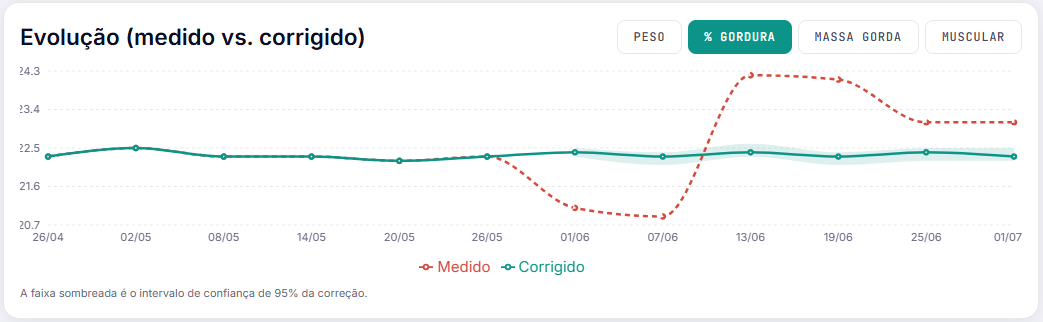
\includegraphics[width=.92\linewidth]{figuras/grafico-correcao-gordura}\\[.15cm]
    {\footnotesize (a) percentual de gordura}\\[.45cm]
    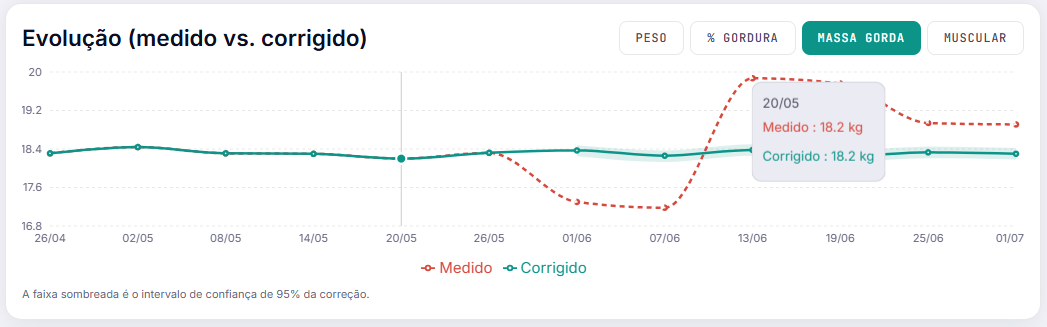
\includegraphics[width=.92\linewidth]{figuras/grafico-correcao-massagorda}\\[.15cm]
    {\footnotesize (b) massa gorda}\\[.45cm]
    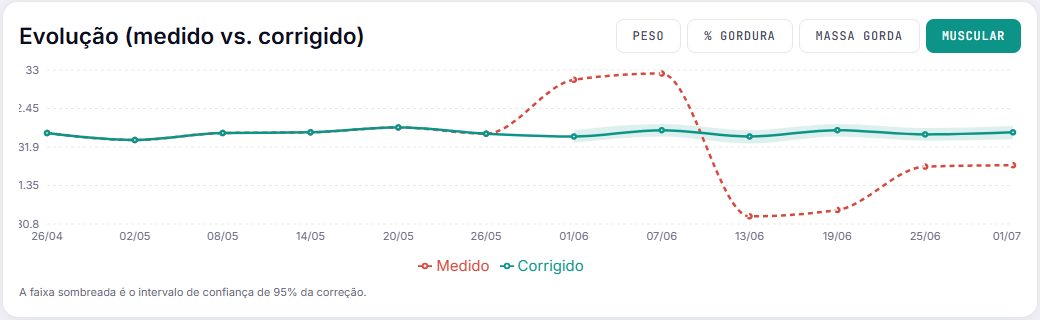
\includegraphics[width=.92\linewidth]{figuras/grafico-correcao-muscular}\\[.15cm]
    {\footnotesize (c) massa muscular esquelética}
    \caption{Gráfico de evolução do \sintonia\ para três métricas: a linha ``medido'' oscila
    conforme o contexto de cada medição, enquanto a linha ``corrigido'' permanece estável; a
    faixa sombreada é o intervalo de confiança de 95\% da correção \emph{within-user}.}
    \label{fig:grafico-correcao}
\end{figure}

\tabela{Estudo de simulação da correção \emph{within-user}: viés injetado por confundidor e viés recuperado pelo modelo (impedância de 50~kHz)}{tab:correcao}{lcc}{%
    \toprule
    Confundidor & Viés injetado ($\Omega$) & Viés recuperado ($\Omega$) \\
    \midrule
    Não estava em jejum & $+8{,}0$  & $+9{,}1$  \\
    Ingeriu água        & $-18{,}0$ & $-16{,}0$ \\
    Exercício recente    & $+25{,}0$ & $+27{,}1$ \\
    \bottomrule
}

Esses testes, ainda que preliminares e conduzidos com um número reduzido de medições,
demonstraram o funcionamento integrado dos módulos do \sintonia\ e a viabilidade técnica da
solução. A avaliação quantitativa com usuários e a validação por especialistas permanecem
como trabalho futuro (Capítulo~\ref{cap:trabalhosfuturos}).

\section{Considerações sobre a Implementação}

O desenvolvimento do \sintonia\ mostrou que é viável integrar dispositivos de bioimpedância,
processamento computacional e modelos de linguagem executados localmente. A arquitetura
permitiu adquirir, armazenar, interpretar e apresentar os dados de composição corporal em
uma única plataforma, com privacidade, transparência e controle dos dados pelo usuário.
Algumas funcionalidades ainda estão em evolução, mas os resultados mostram que a solução é
útil para acompanhamento corporal e saúde digital e pode servir de base para trabalhos
futuros.
